\section{Resultados}


Para criar o modelo do sistema solar tomaram-se algumas liberdades em relação
à distância dos planetas ao Sol, e como tal os valores das translações são mais
ou menos obtidos por experimentação. Não obstante,  os planetas estão colocados
sobre o eixo dos \emph{xx}. Para as órbitas, teve-se que ter em conta
o raio interior do anel (como o anel é bastante fino, é redundante calcular
o valor médio), e fazer uma escala ao anéis, é preciso dividir a distância
à origem, pelo valor do raio interior do anel. As rotações tiveram como base
valores reais, sendo o eixo de rotação o vetor (0,0,1).


Os resultados obtidos estão nas imagens seguintes.


A \emph{Figura~\ref{fig:ssec3:ptl}} mostra o grupo de planetas terrestres e lua
da Terra. 

\begin{center}
 	
 	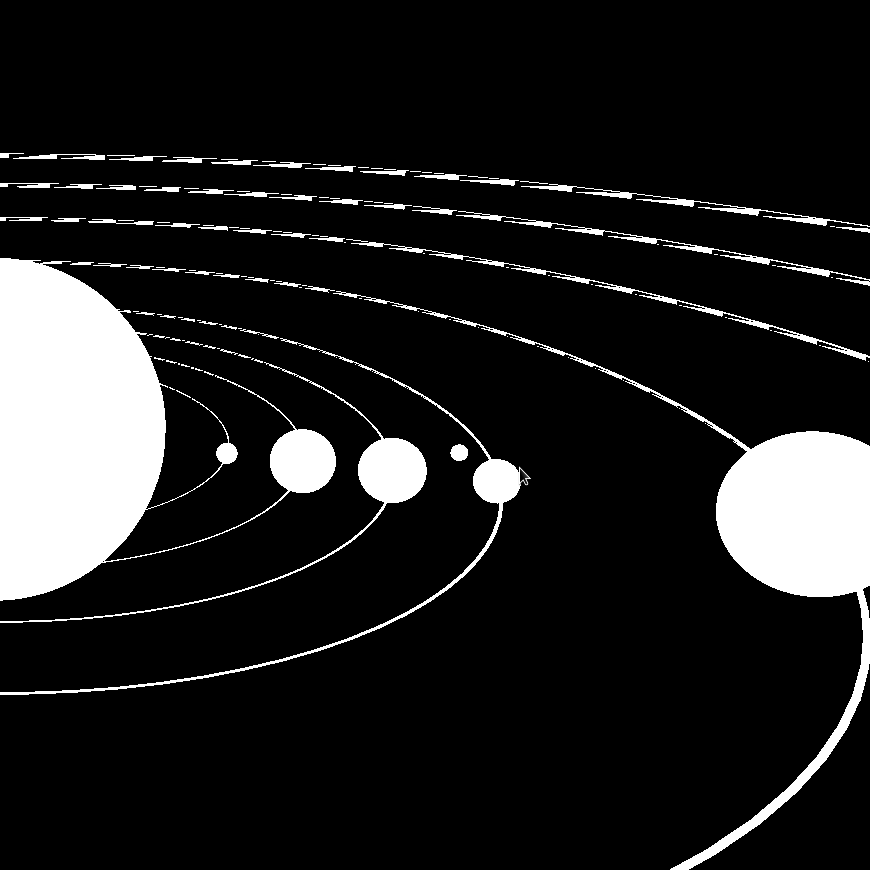
\includegraphics[width=\textwidth,height=\textheight,keepaspectratio]{resources/pormenorTerrestres.png}
 	\captionsetup{type=figure, width=0.8\linewidth}
	\caption{\textit{Rendering} do modelo com foco do grupo de planetas terrestres e Lua}
\label{fig:ssec3:ptl} 
\end{center}


A \emph{Figura~\ref{fig:ssec3:tilt}} mostra Urano e Neptuno, com o \emph{tilt}
axial aplicado. 

\begin{center}
 	
 	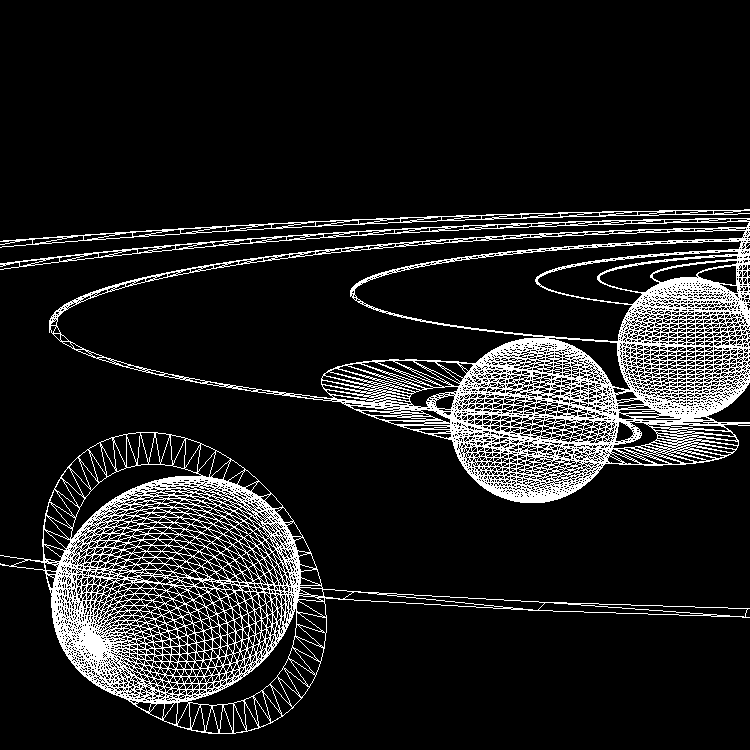
\includegraphics[width=\textwidth,height=\textheight,keepaspectratio]{resources/pormenorTiltAxial.png}
 	\captionsetup{type=figure, width=0.8\linewidth}
	\caption{\textit{Rendering} do modelo com foco no \textit{tilt} axial de Urano e Neptuno}
\label{fig:ssec3:tilt} 
\end{center}


A \emph{Figura~\ref{fig:ssec3:modelo}} mostra o modelo completo. 

\begin{center}
 	
 	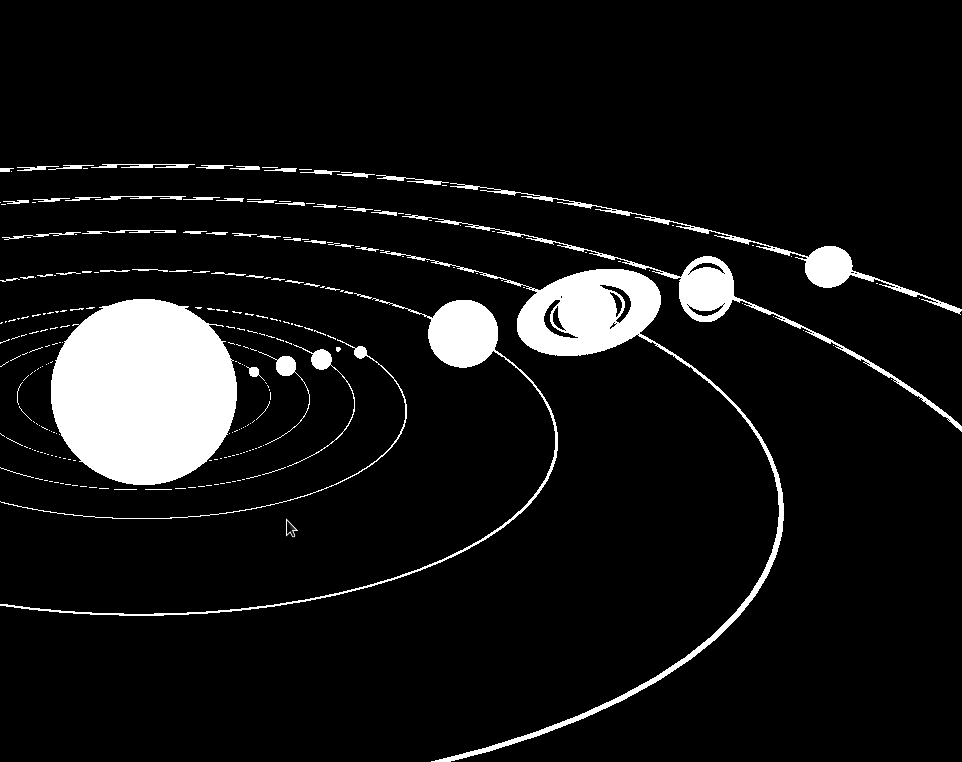
\includegraphics[width=\textwidth,height=\textheight,keepaspectratio]{resources/modelo.png}
 	\captionsetup{type=figure, width=0.8\linewidth}
	\caption{\textit{Rendering} do modelo final}
\label{fig:ssec3:modelo} 
\end{center}
